\documentclass{article}

\usepackage{ragged2e}
\usepackage{graphicx}
\usepackage{amsmath}
\usepackage{siunitx}

\begin{document}
    
\begin{flushright}
    \noindent
    Rodrigo Becerril Ferreyra\\
    CECS 211 Section 01\\
    Lab 2\\
    2019-09-12--2019-09-17
\end{flushright}

\textbf{Question 1}

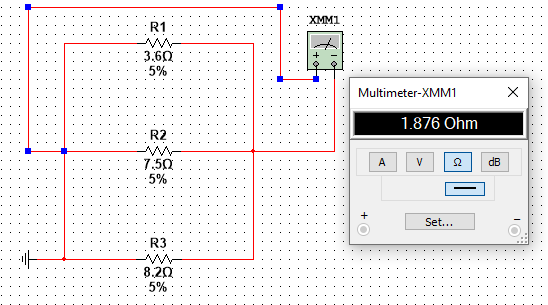
\includegraphics[width=\textwidth]{Lab3Screenshot1.png}

This multimeter reads \SI{1.876}{\ohm}. This is because it is reading the
resistances of the three resistors (from top to bottom:
$R_1 = \SI{3.600}{\ohm}$,
$R_2 = \SI{7.500}{\ohm}$, and
$R_3 = \SI{8.200}{\ohm}$)
that are in parallel. The formula to calculate the effective value of
all three resistors is as follows:

\begin{equation}
    R_{\text{net}} = \left( \sum_{i=1}^n \frac1{R_i} \right)^{-1}
\end{equation}

Using formula (1) with the above values for $R_1$, $R_2$, and $R_3$ gives
us the following result:

\begin{align*}
    R_{\text{net}}
    &= \left( \frac1{R_1} + \frac1{R_2} + \frac1{R_3} \right)^{-1}\\ 
    &= \left( \frac{1}{\SI{3.600}{\ohm}} + \frac1{\SI{7.500}{\ohm}} + \frac1{\SI{8.200}{\ohm}} \right)^{-1}\\ 
    &= \left( \SI{0.278}{\per\ohm} + \SI{0.133}{\per\ohm} + \SI{0.122}{\per\ohm} \right)^{-1}\\
    &= \left(\SI{0.533}{\per\ohm}\right)^{-1}\\
    &= \SI{1.876}{\ohm}
\end{align*}

\pagebreak

\textbf{Question 2}

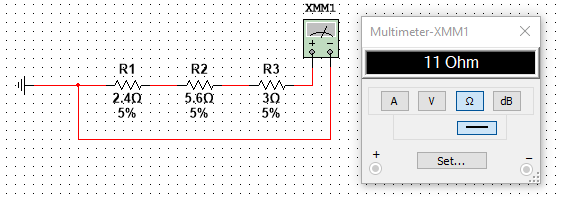
\includegraphics[width=\textwidth]{Lab3Screenshot2.png}

This multimeter reads \SI{11}{\ohm}. This is because the three resistors are
connected in series
    ($R_1 = \SI{2.4}{\ohm}$,
    $R_2 = \SI{5.6}{\ohm}$, and
    $R_3 = \SI{3.0}{\ohm}$).
When resistors are connected in series, the equivalent resistance is simply
the sum of all the resistances: $R_{\text{net}} = \sum_{i=1}^n R_i$.

\begin{align*}
    R_{\text{net}} &= R_1 + R_2 + R_3\\ 
    &= \SI{2.4}{\ohm} + \SI{5.6}{\ohm} + \SI{3.0}{\ohm}\\ 
    &= \SI{11}{\ohm}
\end{align*}

\textbf{Question 3}

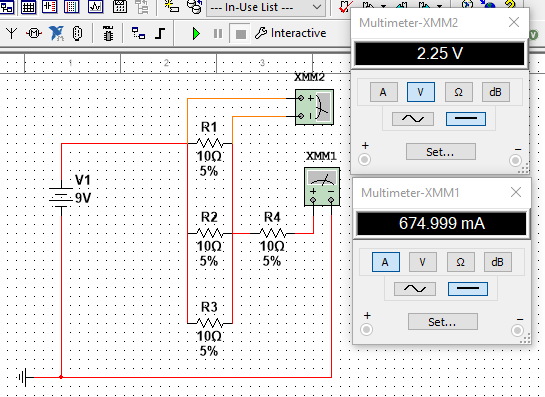
\includegraphics[width=\textwidth]{Lab3Screenshot3.png}

In this example, XMM1 (reading current) reads \SI{674.999}{\milli\ampere} (which
can be rounded up to \SI{675.000}{\milli\ampere}, or \SI{0.675}{\ampere})
and XMM2 (reading voltage) reads \SI{2.25}{\volt}.
To calculate these values, it is first necessary
to calculate the total effective resistance $R_{\text{net}}$. In this complex
example, three resistors ($R_1 = R_2 = R_3 = \SI{10}{\ohm}$) are placed in
parallel with each other, while one more resistor ($R_4 = \SI{10}{\ohm}$) is
placed in series with the other three. First, it is required to calculate the
effective total resistance of $R_1$, $R_2$, and $R_3$ together; next, this
intermediate value can be added to $R_4$ to achieve total resistance.

\begin{align*}
    R_{1+2+3}
    &= \left(\sum_{i=1}^n \frac1{R_i} \right)^{-1} = \left( \sum_{i=1}^3 \frac1{\SI{10}{\ohm}} \right)^{-1} \\ 
    &= \left( 3 \times \frac1{\SI{10}{\ohm}} \right)^{-1} = \left( \frac3{\SI{10}{\ohm}} \right)^{-1}\\ 
    &= \SI{3.33}{\ohm}\\ 
    \\
    R_{\text{net}} &= R_{1+2+3} + R_4\\ 
    &= \SI{3.33}{\ohm} + \SI{10}{\ohm}\\ 
    &= \SI{13.33}{\ohm}
\end{align*}

With this quantity, we can determine the values displayed on XMM1 and XMM2.

XMM1 is reading the current going through the whole circuit, because it is
connected to the very end, where there are no nodes or separations. This makes
it possible to use Ohm's Law to calculate the current going through the whole
circuit easily.

\begin{align*}
    V &= IR\\ 
    I &= \frac{V}{R} = \frac{V_s}{R_{\text{net}}}\\ 
    &= \frac{ \SI{9}{\volt} }{ \SI{13.33}{\ohm} }\\
    &= \SI{0.675}{\ampere} = \SI{675}{\milli\ampere}
\end{align*}

XMM2 is reading the voltage going across $R_1$, $R_2$, and $R_3$, which are
connected in parallel. We can combine these three resistances into a single
equivalent resistance (the quantity $R_{1+2+3}$, which was calculated
earlier), and then use Ohm's Law to solve for the voltage going through
all three resistors.

\begin{align*}
    V &= IR\\
    V_{R_{1+2+3}} &= I_{\text{net}} \cdot R_{1+2+3}\\
    &= \SI{0.675}{\ampere} \cdot \SI{3.33}{\ohm}\\
    &= \SI{2.25}{\volt}
\end{align*}

\textbf{Question 4}

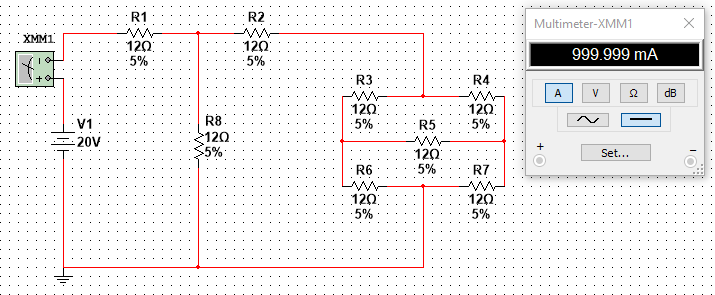
\includegraphics[width=\textwidth]{Lab3Screenshot4.png}

Using Ohm's Law, the equivalent resistance for this resistor network
can be found algebraically if and only if both the total voltage and the
total current are known for the entire circuit. The total voltage is
\SI{20}{\volt}, and the total current (as given by XMM1) is
\SI{999.999}{\milli\ampere}, or \SI{1}{\ampere}.

\begin{align*}
    V &= IR \Rightarrow R = V/I\\
    R_{\text{net}} &= \frac{V_s}{I_{\text{net}}}\\
    &= \frac{ \SI{20}{\volt} }{ \SI{1}{\ampere} }\\
    &= \SI{20}{\ohm}
\end{align*}

\textbf{Question 5}

\textit{Problem 1}

$R_3 = \SI{20}{\ohm}$ and $R_4 = \SI{20}{\ohm}$ are connected in parallel,
while $R_1 = \SI{10}{\ohm}$ and $R_2 = \SI{15}{\ohm}$ are connected in
series with $R_3 + R_4$. This means that it is necessary to calculate
$R_{3+4}$ before adding it to $R_1$ and $R_1$ and $R_2$.

\begin{align*}
    R_{3+4} &= \left( \sum_{i=3}^4 \frac1{R_i} \right)^{-1}\\
    &= \left( 2 \times \frac1{\SI{20}{\ohm}} \right)^{-1}
    = \left( \frac1{\SI{10}{\ohm}} \right)^{-1} \\
    &= \SI{10}{\ohm}
\end{align*}
\begin{align*}
    R_{\text{net}} &= R_1 + R_2 + R_{3+4}\\
    &= \SI{10}{\ohm} + \SI{15}{\ohm} + \SI{10}{\ohm}\\
    &= \SI{35}{\ohm}
\end{align*}

The equivalent resistance is \SI{35}{\ohm}.

\indent\textit{Problem 2}

In this problem, $R_7 = \SI{20}{\ohm}$ and $R_8 = \SI{15}{\ohm}$ are
connected in parallel, and this combo $R_{7+8}$ is connected in series with
$R_5 = \SI{7.5}{\ohm}$.

\begin{align*}
    R_{\text{net}} &= R_5 + R_{7+8}\\
    &= \SI{7.5}{\ohm} + \left( \frac1{\SI{20}{\ohm}} + \frac1{\SI{15}{\ohm}} \right)^{-1}\\
    &= \SI{7.5}{\ohm} + \left( \SI{0.05}{\per\ohm} + \SI{0.067}{\per\ohm} \right)^{-1}\\
    &= \SI{7.5}{\ohm} + \left( \SI{0.117}{\per\ohm} \right)^{-1}\\
    &= \SI{7.5}{\ohm} + \SI{8.55}{\ohm}\\
    &= \SI{16.047}{\ohm}
\end{align*}

The equivalent resistance is \SI{16.047}{\ohm}.

\indent\textit{Problem 3}

The resistors in this network are situated such that $R_{13}$ and the
rest of the resistors (which I will call $R_a$) are connected in parallel.
$R_a$ consists of $R_{10}$ and $R_{11}$ in parallel plus $R_6$ and $R_{12}$ in
parallel plus $R_9$ in series.

%\begin{align*}
%   R_{\text{net}} &= {1 \over \frac{1}{R_{13}} + \frac{1}{R_a}} \\
%   &= \frac{1}{\frac{1}{R_{13}}+\frac{1}{\frac{1}{\frac{1}{R_{10}}+\frac{1}{R_{11}}}+\frac{1}{\frac{1}{R_6}+\frac{1}{R_{12}}} + R_9}}\\
%    &= \frac{1}{\frac{1}{\SI{10}{\ohm}}+\frac{1}{\frac{1}{\frac{1}{\SI{10}{\ohm}}+\frac{1}{\SI{15}{\ohm}}}+\frac{1}{\frac{1}{\SI{6.8}{\ohm}}+\frac{1}{\SI{13.0}{\ohm}}}+\SI{5.1}{\ohm}}}\\
%    &= {1 \over \SI{0.1}{\per\ohm} + {1 \over {1 \over \SI{0.1}{\per\ohm} + \SI{0.067}{\per\ohm} } + {1 \over \SI{0.147}{\per\ohm} + \SI{0.077}{\per\ohm} } + \SI{5.1}{\ohm} } }\\
%    &= {1 \over \SI{0.1}{\per\ohm} + {1\over \frac1{\SI{0.167}{\per\ohm}} + \frac1{\SI{0.224}{\per\ohm}} + \SI{5.1}{\ohm} } }\\
%    &= {1 \over \SI{0.1}{\per\ohm} + {1 \over \SI{5.988}{\ohm} + \SI{4.464}{\ohm} + \SI{5.1}{\ohm} } }\\
%    &= \frac{1}{ \SI{0.1}{\per\ohm} + \frac{1}{ \SI{15.552}{\ohm} } }\\
%    &= \frac{1}{ \SI{0.1}{\per\ohm} + \SI{0.064}{\per\ohm} } = \frac{1}{\SI{0.164}{\per\ohm}}\\
%    &= \SI{6.098}{\ohm}
%\end{align*}

%\pagebreak

\begin{align*}
    R_{\text{net}} &= \left( \frac1{R_{13}} + \left( R_a \right)^{-1} \right)^{-1}\\
    &= \left( \frac1{R_{13}}        + \left( \left( \frac1{R_{10}} + \frac1{R_{11}} \right)^{-1} +               \left( \frac1{R_6} + \frac1{R_{12}} \right)^{-1} + R_9 \right)^{-1} \right)^{-1}\\
    &= \left( \frac1{\SI{10}{\ohm}} + \left( \left( \frac1{\SI{10}{\ohm}} + \frac1{\SI{15}{\ohm}} \right)^{-1} + \left( \frac1{\SI{6.8}{\ohm}} + \frac1{\SI{13}{\ohm}}  \right)^{-1} + \SI{5.1}{\ohm} \right)^{-1}  \right)^{-1}\\
    &= \left( \SI{0.1}{\per\ohm} + \left( \SI{6}{\ohm} + \SI{4.465}{\ohm} + \SI{5.1}{\ohm} \right)^{-1} \right)^{-1}\\
    &= \left( \SI{0.1}{\per\ohm} + \SI{0.0642}{\per\ohm} \right)^{-1}\\
    &= \SI{6.088}{\ohm}
\end{align*}

The equivalent resistance is \SI{6.088}{\ohm}.

\pagebreak

\indent\textit{Problem 4}

Here, $R_{14} = \SI{100}{\ohm}$ and $R_{17} = \SI{100}{\ohm}$ are in series,
and $R_{15} = \SI{100}{\ohm}$ and $R_{17} = \SI{100}{\ohm}$ are in
series, and these two groups are connected in parallel with
$R_{19} = \SI{100}{\ohm}$.

\begin{align*}
    R_{\text{net}} &= (R_{14} + R_{17}) \parallel R_{19} \parallel (R_{15} + R_{18})\\
    &= (\SI{100}{\ohm} + \SI{100}{\ohm}) \parallel \SI{100}{\ohm} \parallel (\SI{100}{\ohm} + \SI{100}{\ohm})\\
    &= \SI{200}{\ohm} \parallel \SI{100}{\ohm} \parallel \SI{200}{\ohm}\\
    &= {1 \over \frac1{\SI{200}{\ohm}} + \frac1{\SI{100}{\ohm}} + \frac1{\SI{200}{\ohm}}}\\
    &= {1 \over \SI{0.005}{\per\ohm} + \SI{0.01}{\per\ohm} + \SI{0.005}{\per\ohm}}\\
    &= {1 \over \SI{0.02}{\per\ohm}} = \SI{50}{\ohm}
\end{align*}

The equivalent resistance is \SI{50}{\ohm}.

\end{document}
